% \begin{figure}[t]
% \centering
% 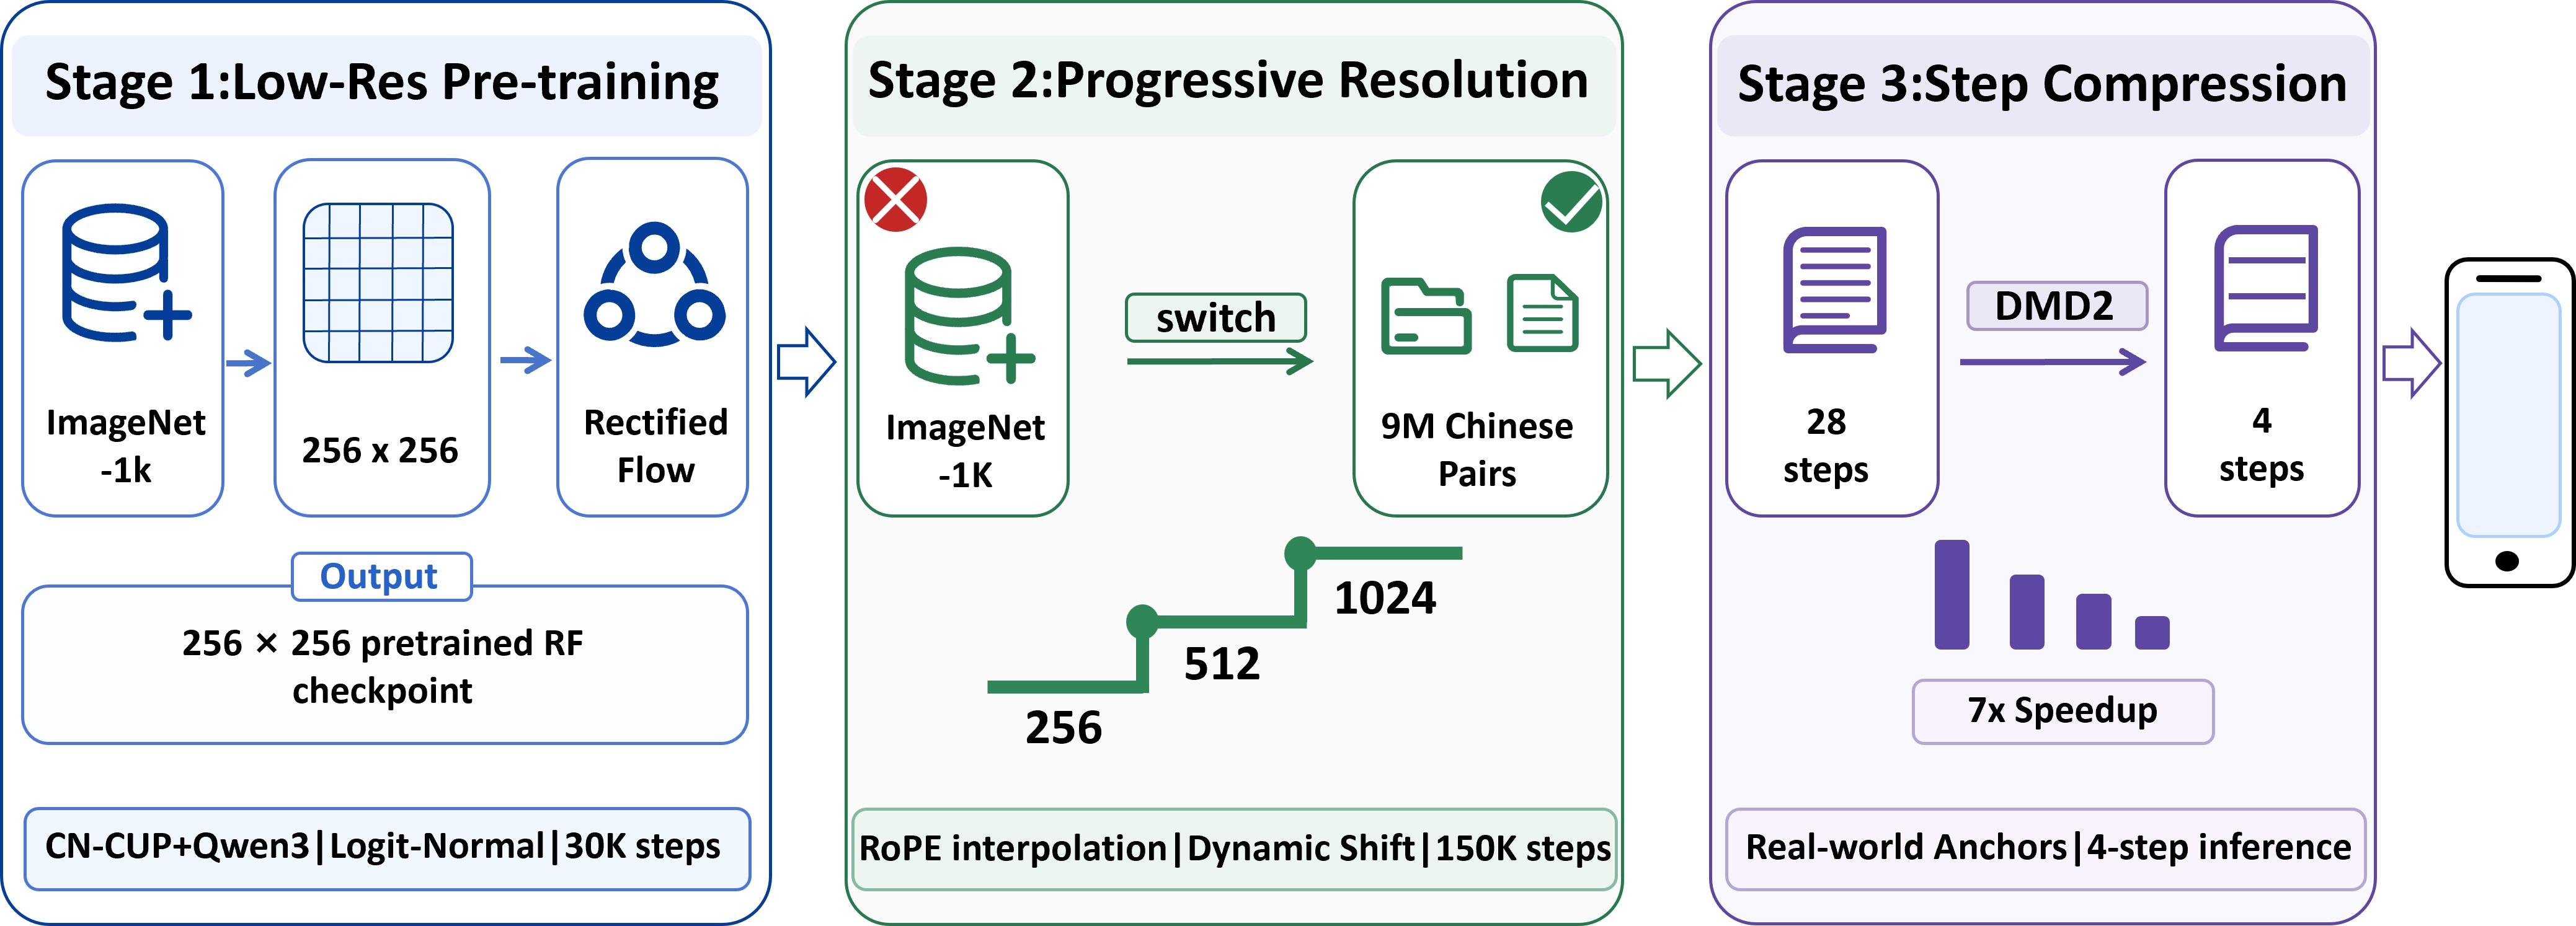
\includegraphics[width=\textwidth]{figures/figures/003.jpg}
% \caption{\textbf{The multi-stage training framework of JuZhou 1.0.} Stage~1 establishes foundational visual representations at $256\times256$ using ImageNet-1K with Rectified Flow and a dual text encoder. Stage~2 progressively scales resolution to $1024\times1024$ while transitioning to 9M Chinese image-text pairs. Stage~3 compresses the inference trajectory from 28 to 4 steps via DMD2 distillation, achieving $7\times$ latency reduction.}
% \label{fig:training_framework}
% \end{figure}

% \section{Multi-stage Training Framework}

% The training of JuZhou 1.0 follows a carefully designed multi-stage pipeline that systematically builds generative capability from low to high resolution before compressing the inference trajectory. This staged approach serves two purposes: it reduces overall computational cost by establishing foundational visual representations at low resolution, and it ensures stable convergence when scaling to the target $1024 \times 1024$ output. The framework comprises three successive stages---low-resolution pre-training, progressive resolution scaling, and inference step compression---each building upon the previous stage while introducing a distinct optimization dimension (data scale, spatial detail, and inference speed, respectively).

% \subsection{Low-Resolution Pre-training}

% Training diffusion models directly at high resolution demands enormous computational resources and is prone to convergence instability. We therefore adopt a staged approach that begins with low-resolution pre-training to establish robust visual representations before scaling to higher resolutions. We begin training at $256 \times 256$ resolution on ImageNet-1K~\cite{deng2009imagenet}, pairing each image with a class-conditional text template. This stage is designed to endow the denoising network with fundamental visual priors, including object structure, color coherence, and spatial layout, at minimal computational cost.

% A distinctive aspect of our pre-training stage is the adoption of the \textit{Rectified Flow}~\cite{liu2022flow} formulation from the outset, rather than starting with a conventional DDPM objective and subsequently switching paradigms. This unified training objective eliminates distributional drift caused by paradigm transitions and ensures that the learned velocity field remains consistent across all subsequent training stages. To capture the semantic content of each class, we employ a dual text-encoder architecture combining CN-CLIP~\cite{chinese-clip,radford2021clip} with Qwen3~\cite{qwen3technicalreport}. Although the ImageNet captions are English class names, this dual-encoder design pre-aligns the text conditioning pathway with the Chinese semantic space, facilitating a seamless transition to Chinese-centric data in later stages, building upon prior work in Chinese text-to-image synthesis~\cite{ding2021cogview}. For timestep scheduling, we adopt logit-normal sampling with dynamic timestep shifting, which concentrates training effort on intermediate noise levels that are most informative for the denoising objective.

% To maximize training throughput on domestic Sugon K100 clusters, we implement a feature pre-computation strategy that caches text embeddings and image latents in advance, substantially reducing per-iteration data loading overhead. The pre-training is conducted on 56 nodes (4 accelerators per node) with a per-accelerator batch size of 512 (global batch size of 114{,}688) for 30K steps, using a learning rate of $3 \times 10^{-4}$ with the AdamW optimizer.

% \subsection{Progressive Resolution Increasing}

% After the low-resolution foundation is established, we progressively increase the training resolution from $256 \times 256$ through $512 \times 512$ to the target $1024 \times 1024$. Training directly at high resolution from scratch is both computationally prohibitive and prone to mode collapse; a gradual resolution schedule allows the model to refine coarse-grained features into fine-grained details while maintaining stable optimization dynamics. At each resolution transition, we apply interpolation to the 2D Rotary Position Embedding (RoPE)~\cite{su2024roformer}, enabling the position encodings to adapt smoothly to the expanded spatial dimensions without re-initialization.

% A critical design choice at this stage is the transition in training data. While the low-resolution pre-training relies on ImageNet-1K for acquiring universal visual concepts, the progressive resolution stage switches to our curated 9M Chinese image-text pairs. This data transition serves two purposes: it introduces native Chinese semantic alignment at scale, and it exposes the model to the diverse, high-quality aesthetic content required for photorealistic synthesis. The logit-normal timestep sampling is accompanied by a dynamic shift factor that increases with resolution, compensating for the lower signal-to-noise ratio inherent in high-resolution latent spaces.

% The resolution-increasing stage is trained on the same 56-node Sugon K100 cluster with a per-accelerator batch size of 12 (global batch size of 2{,}688), a learning rate of $1.0 \times 10^{-4}$, and 150K total training steps. The feature pre-computation strategy continues to be applied throughout this stage, maintaining the training efficiency gains established during pre-training.

% \subsection{Inference Step Compression}

% To enable real-time text-to-image generation on mobile devices while preserving visual quality, we develop an aggressive inference step compression strategy for our Flow Matching-based model~\cite{luo2023lcm,lin2024sdxl_lightning,sauer2024ladd,sauer2023conditioning}. The original model requires 28 sampling steps to produce high-quality images, imposing a substantial latency overhead for on-device deployment. Through step distillation~\cite{yin2024improved_dmd,luo2023lcm_loRA}, we compress the generation process to only 4 steps, achieving a $7\times$ reduction in end-to-end inference latency and making near-instantaneous image synthesis feasible on mobile platforms.

% Our method combines the core idea of Distribution Matching Distillation (DMD2) with iterative step distillation, adapted to the Flow Matching setting. By incorporating real-world samples as distributional anchors during training, the student model is guided toward more realistic texture, lighting, and structural statistics rather than merely approximating the teacher's deterministic ODE path.
% This design substantially improves both efficiency and image fidelity. In addition to the significant latency reduction from 28 steps to 4, the distilled model delivers a notable improvement in visual quality over the baseline distilled counterpart. Qualitatively, we observe improved recovery of fine-grained textures, more natural illumination transitions, and overall more photorealistic outputs. These gains suggest that introducing real data into the distillation process is critical for overcoming the limitations of synthetic-heavy supervision, enabling the compressed model to remain both efficient enough for mobile deployment and faithful to high-quality image generation.
